\documentclass[en]{../../../eplsummary}

\usepackage{listings}


\lstset{
  frame=top,frame=bottom,
  basicstyle=\footnotesize\normalfont\sffamily,    % the size of the fonts that are used for the code
  stepnumber=1,                           % the step between two line-numbers. If it is 1 each line will be numbered
  numbersep=10pt,                         % how far the line-numbers are from the code
  tabsize=2,                              % tab size in blank spaces
  extendedchars=true,                     %
  breaklines=true,                        % sets automatic line breaking
  captionpos=t,                           % sets the caption-position to top
  mathescape=true,
  stringstyle=\color{white}\ttfamily, % Farbe der String
  showspaces=false,           % Leerzeichen anzeigen ?
  showtabs=false,             % Tabs anzeigen ?
  xleftmargin=17pt,
  framexleftmargin=17pt,
  framexrightmargin=17pt,
  framexbottommargin=5pt,
  framextopmargin=5pt,
  showstringspaces=false      % Leerzeichen in Strings anzeigen ?
 }

\DeclareCaptionFormat{listing}{\rule{\dimexpr\textwidth+17pt\relax}{0.4pt}\par\vskip1pt#1#2#3}
\captionsetup[lstlisting]{format=listing,singlelinecheck=false, margin=0pt, font={sf},labelsep=space,labelfont=bf}

\renewcommand\lstlistingname{Algorithm}

\tikzset{
r/.style = {treenode, circle, text width=1.5em, very thick}
}

\hypertitle{Constraint Programming}{8}{INGI}{2365}
{Houtain Nicolas}
{Yves Deville}

\section{Constraint Programming (CP)}
\textsc{CP = Model + Search}

\begin{enumerate} 
    \item \textsc{Model} : Describe real world problem with
        \begin{itemize}
            \item \textbf{Variables} : $X = \{x_1, x_2,\cdots, x_n\}$
            \item \textbf{Domains} : $D = \{ D(x_1), D(x_2),\cdots,
                D(x_n)\}$

                \begin{itemize}
                    \item[Ex:] Booleans, \textbf{finite domains}, finite
                        set, intervals, continuous domains,\ldots
                \end{itemize}
            \item \textbf{Constraints} : $C = \{c_1, c_2,\cdots, C_e\}$
                \begin{itemize}
                    \item A \textbf{scope} $scp(c) = (x_1, x_2,\cdots,x_r)$ : is the
                        variables constrained by c.
                    \item A \textbf{relation} $rel(c)$ : value combinations accepted by
                        c
                \end{itemize}
            \item \textbf{Objective function} : $O = solution \to \R$
        \end{itemize}

        \paragraph{Types}
        \begin{enumerate}
            \item CSP = (X, D, C)
            \item COP = (X, D, C, O)
        \end{enumerate}

        \paragraph{Declarative} : describe what you want not how to get it
    \item[+]
    \item \textsc{Search} : Describe how to solve the problem.
        \begin{itemize}
            \item \textbf{Propagation} : Use constraints to remove
                \textit{useless} (doesn't remove solution) parts of the search space
                \begin{center}
                    \scriptsize
                    \textit{Need choice between more pruning with more
                        expensive to compute or less proning cheaper to
                    compute}
                \end{center}

                \begin{itemize}
                    \item Consistencies : Require that all the values
                        are able to satisfy their constaints in
                        \textbf{isolation}

                    \item Propagator: used at the beginning of the search
                        and each time a decision is made.
                \end{itemize}
            \item \textbf{Backtrackink Tree Search} : Explore search
                space by taking decisions and backtracking (with
                remembering decision)

                \paragraph{Current node}: The node is modified at each decision
                make and he is restore when backtracking occur.
        \end{itemize}

        \paragraph{Search space} = $D(x_1) \times D(x_2) \times \cdots \times D(x_n)$
\end{enumerate}


\paragraph{Solution}
A solution to a CSP is 
\begin{enumerate}
    \item An assigment of variabels ot values in their domains
    \item Such that all the constraints are respected
\end{enumerate}

% TODO ---v %
\subsection{Auxiliary variables}
Variables used to help/improve modeling

Vs

variable which reprendt the decision CP has to make

reducundant constraint : constraint that does not exclude any previous solution,
improve prining (reduce search space), improve communication

\subsection{Global constraint}

\subsection{Symmetry}





\section{Propagation}
\begin{itemize}
    \item $n$ variables
    \item domains of size $d$
    \item $e$ constraints
    \item maximum arity $r$
\end{itemize}

\begin{table}
    \centering
\begin{tabular}{|c|c|c|c|c|}
    \hline
    & Algo & Complexity & Type & Other \\
    \hline
    \hline
    \multirow{3}{*}{\rotatebox{90}{\scriptsize Constraint}}     
    & GAC3 & $O(e \times r^3 \times d^{r+1})$ & n-ary & \\
    & AC3rm & $0(e \times d^3)$ & binary & Residues \& multidirectionality\\
    & AC2001 & $O(e \times d^2)$ & binary &  firstSupport(x, a)\\

    \hline
    \hline
    \multirow{2}{*}{\rotatebox{90}{\scriptsize Value}}
    & GAC4 & $O(e \times r \times d^r)$ & n-ary & c.support(x,a) \\
    & AC6 & $O(e \times d^2)$ & binary & firstSupported(x, a) \\
    \hline
\end{tabular}
\caption{Generic propagator algorithm}
\end{table}

\begin{table}
    \centering
    \begin{tabular}{|m{5cm}|m{5cm}|m{5cm}|}
        \hline
        CB & Collect and propagate & VB \\
        \hline

        c in Q & c in Q & (c, x, a) in Q \\

        \begin{itemize}
            \item called once for each set of change in SP
            \item re-enforce the whole consistency
            \item no information on changes
        \end{itemize}
        &
        &
        \begin{itemize}
            \item called once for each single change in SP
            \item reflects only one change at a time ($a \notin D(c)$)
            \item information on each change, one at a time
        \end{itemize}
        \\

        \hline

        \scriptsize
        \begin{enumerate}
            \item \textcolor{red}{less} information
            \item called \textcolor{green}{less}
        \end{enumerate}
        &
        \scriptsize
        \begin{enumerate}
            \item \textcolor{green}{more} information
            \item called \textcolor{green}{less}
        \end{enumerate}
        &
        \scriptsize
        \begin{enumerate}
            \item \textcolor{green}{more} information
            \item called \textcolor{red}{more}
        \end{enumerate}
        \\

        \multicolumn{3}{|c|}{\begin{tikzpicture}
            \draw[<->] (0,0) -- (13, 0);
        \end{tikzpicture}}\\
        \hline

    \end{tabular}
    \caption{Fixed point}
\end{table}

\subsection{Without propagation (Bruteforce)}:

\begin{tabular}{m{6cm}cm{6cm}}
    \begin{itemize}
        \item $O(d^n)$ possible assignements
        \item $O(r)$ to test a constraint
        \item $O(e \times r)$ to test all constraint
    \end{itemize}
    & $\to$ &
    \textbf{Global complexity}: $O(d^n \times e \times r)$
\end{tabular}

\subsection{Fonctionnement}

The goal of propagation is to \textbf{reduce} the search space
(\textit{reduction domains, reduction constraints, addition constraint})
but do not remove solutions.

The propagation is used before the search and all along the search.

\subsubsection{Partial solution} 

A partial instantiation gives values to some variables.
It's a \textbf{partial solution} IFF
\begin{center}
    for all constraint c : if all variables assigned $\to$ c satisfied  
\end{center}


The propagation perfom checking and \textcolor{red}{fail} when there is
no partial solution : checking fails or there is inconsistency (empty domain,\ldots)

\subsubsection{Level of propagation}
\begin{tabular}{ccc}
    \textbf{Weaker} & $\Rightarrow$ & \textbf{Stronger} \\
    Less pruning & & More pruning \\
    Cheaper to compute & & More expensive to compute \\
\end{tabular}


\subsection{Constraint based propagation}

\subsubsection{Fixed point algorithm}

The propagator must implements two methods :
\begin{enumerate}
    \item setup() : initialize the constraint
    \item propagate() : compute the set of values that are inconsistent

    \item[Note:] removeValue(a, D(x)) fails if D(x) empty
\end{enumerate}

\paragraph{Note:} use GAC consistency

\begin{lstlisting}[mathescape, caption=CB Fixed point]
initCBDomFilter(Q){
    for(c $\leftarrow$ C){
        c.setup()
        Q += c
    }
}

CBDomFilter(X, D, C){
    Q = $\emptyset$
    initCBDomFilter(Q)
    propagateQueueCBDomFilter(Q)
}

propagateQueueCBDomFilter(Q){
    while(Q $\neq$ $\emptyset$){
        c = popCtrt(Q)
        $\Delta$ = c.propagate()
        for((x,a) $\leftarrow$ $\Delta$){
            removeValue(a,D(x))             
            for(c $\leftarrow$ C/{c} if c.scope contains x){
                if(! Q contains c)
                    Q += c
            }
        }
    }
}

\end{lstlisting}

\subsubsection{Generic GAC}

The only requirement is a test method for the constraint which say true/false
if the given value is right.


\begin{enumerate}
    \item \textbf{GAC3} \begin{lstlisting}[mathescape, caption=GAC3]
setup(){}

propagate(){
    $\Delta$ = $\emptyset$
    for(x $\leftarrow$ scope){
        for(a $\leftarrow$ D(x)){
            if( $\forall(v \leftarrow D(scope)_{x=a}) (! c(v))$ )
                // No combination with x=a satisfying the constraint in the current dom
                $\Delta$ += (x, a)
        }
    }
    return $\Delta$
}
    \end{lstlisting}

    \begin{tabular}{m{7cm}cm{6cm}}
        \begin{itemize}
            \item $O(r^2 \times d^r)$ for propagate()
            \item $O(r \times d)$ calls of propagate() in propagateQueueCBDomFilter
        \end{itemize}
        & $\to$ &
        \textbf{Global complexity}: $O(e \times r^3 \times d^{r+1})$
    \end{tabular}

\item \textbf{AC3rm} : the idea is to add memory by check the last found
    support first. 
    \paragraph{AC3 with }
    \begin{itemize}
        \item Residues :  \texttt{c.support(x, a)} = last found support for (x, a)
            
        \item Multidirectionality : if $b$ is a support for $a$, then $a$ is 
            a support for $b$
    \end{itemize}

\paragraph{Note: } Propagator for binary constraints ($scp(c)=(x, y)$)

\begin{lstlisting}[mathescape, caption=AC3rm]
setup(){
    for(a $\leftarrow D(x)$) { support(x, a) = $\bot$}
    for(b $\leftarrow D(y)$) { support(y, b) = $\bot$}

propagate(){
    $\Delta_1$ = propagate_var(x)
    $\Delta_2$ = propagate_var(y)
    return $\Delta_1 \cup \Delta_2$
}

propagate_var(x){
    $\Delta$ = $\emptyset$
                            // Residues
    for(a $\leftarrow$ D(x) if (! D(y) contains support(x, a))){
        b = y.min
        while(b != $\top$ && ! c(x=a, y=b)){
            b = y.valueAfter(b)
        }
        if( b == $\top$ )
            $\Delta$ += (x, a)
        else {
            // Multidirectionality
            support(x, a) = b
            support(y, b) = a            
        }
    }

    return $\Delta$
}
    \end{lstlisting}

    \begin{tabular}{m{7cm}cm{6cm}}
        \begin{itemize}
            \item $O(d)$ for setup()
            \item $O(d^2)$ for propagate()
            \item $O(d)$ calls of propagate() in propagateQueueCBDomFilter
        \end{itemize}
        & $\to$ &
        \textbf{Global complexity}: $O(e \times d^3)$
    \end{tabular}

    \paragraph{Backtrack}: when we backtrack, AC3rm only search support for
    values that have lost theirs. When needed, the backtracking scan \textbf{all
    the domain} of the other variable!

    $\to$ AC2001 to optimise the backtracking

\item \textbf{AC2001} : to avoid to scan \textit{all the domain}, a node
keep the firstSupport which may be restore when backtracking.

\paragraph{Note: } Propagator for binary constraints ($scp(c)=(x, y)$)

\begin{lstlisting}[mathescape, caption=AC3rm]
setup(){
    for(a $\leftarrow D(x)$) { support(x, a) = $\bot$}
    for(b $\leftarrow D(y)$) { support(y, b) = $\bot$}

propagate(){
    $\Delta_1$ = propagate_var(x)
    $\Delta_2$ = propagate_var(y)
    return $\Delta_1 \cup \Delta_2$
}

propagate_var(x){
    $\Delta$ = $\emptyset$
                            // Residues
    for(a $\leftarrow$ D(x) if (! D(y) contains support(x, a))){
        b = y.valueAfter(firstSupport(x,a))
        while(b != $\top$ && ! c(x=a, y=b)){
            b = y.valueAfter(b)
        }
        firstSupport(x, a) = b

        if( b == $\top$ )
            $\Delta$ += (x, a)
    }

    return $\Delta$
}
\end{lstlisting}

\begin{tabular}{m{7cm}cm{6cm}}
    \begin{itemize}
        \item $O(d)$ for setup()
        \item $O(d)$ for one literal, all updates of firstSupport
        \item $O(d)$ for one literal, validity of firstSupport checked
        \item $O(d^2)$ for propagate()
    \end{itemize}
    & $\to$ &
    \textbf{Global complexity}: $O(e \times d^2)$
\end{tabular}

\end{enumerate}

\subsubsection{Specific}
We can improme the previous complexity if we have a propagator specific
for a constraint.

\begin{lstlisting}[caption=Specific propagator for x <= y + k, mathescape]
propagate(){
    $\Delta$ = $\emptyset$
    a = x.max
    while(a != $\bot$ && a > y.max + k){
        $\Delta$ += (x, a)
        a = x.valueBefore(a)
    }

    b = x.min
    while(b != $\bot$ && b < x.min - k){
        $\Delta$ += (y, b)
        b = x.valueAfter(b)
    }

    return $\Delta$
}
\end{lstlisting}


\subsection{Value based propagation}

In this case, the queue contains constraints and literals $(c,x,a)$.
In this case, c has to reflect that $a \notin$ D(x).

\paragraph{ }
\begin{itemize}
    \item[+] efficient filtering
    \item[-] called for each literal removed
\end{itemize}


\paragraph{Treat inconsistent values because $a \notin D(x)$}
c considers (c, y, b) on Q are sill in the domains!

\begin{itemize}
    \item $\gamma$ on X is \textbf{valid} iff $\forall$ x $\in$ X : $\gamma(x) \in D(x)$
    \item $\gamma$ on X is \textbf{Q-valid} iff $\forall$ x $\in$ X : $\gamma(x) \in D(x) 
        \cup \{a: (c, x, a) \in Q\}$
\end{itemize}


\subsubsection{Fixed point algorithm}
In this case, the propagator must implement :
\begin{enumerate}
    \item setup() : initialize the constraint
    \item valRemove(x, a) : computes the set of values that are
        inconsistent because $a \notin D(x)$
\end{enumerate}

\paragraph{Note:} use GAC consistency

\begin{lstlisting}[mathescape, caption=CB Fixed point]

initVBDomFilter(X, D, C){
    Q = $\emptyset$
    C1 = $\emptyset$
    for(c $\leftarrow$ C){
        $\Delta$ = c.setup()
        for( (x, a) $\leftarrow$ $\Delta$){
            removeValue(a, D(x))
            for( c $\leftarrow$ C1 if c.scope contains x){
                if(! Q contains (c, x, a))
                    Q += (c, x, a)
            }
        }
        C1 += c
    }
}

VBDomFilter(X, D, C){
    Q = $\emptyset$
    initVBDomFilter(Q)
    propagateQueueVBDomFilter(Q)
}

propagateQueueVBDomFilter(Q){
    while(Q $\neq$ $\emptyset$){
        (c, x, a) = popCtrtLiteral(Q)
        $\Delta$ = c.valRemove(x, a)
        for((x,a) $leftarrow$ $\Delta$){
            removeValue(a,D(x))             
            for(c $\leftarrow$ C/{c} if c.scope contains x){
                if(! Q contains (c, x, a))
                    Q += (c, x, a)
            }
        }
    }
}

\end{lstlisting}


\subsubsection{Generic}

\begin{enumerate}
    \item \textbf{GAC4} maintains sets of supports for literals (x,a) :
        \begin{center}
            c.support(x,a) = \{ $\gamma \in D(c.scope, Q, c)_{x=a} : c(\gamma)$\}
        \end{center}

        In this way, we removes Q-invalid support and when no more supports, 
        ce can removed them to D(x).

        \paragraph{Note:} c.support must be backtracked during search

\begin{lstlisting}[mathescape, caption=GAC4]
setup(){
    $\Delta$ = $\emptyset$

    // Initialisation of support data structure
    for(x $\leftarrow$ scope){
        for( a $\leftarrow$ D(x))
            support(x, a) = $\emptyset$
    }
    for($\gamma \leftarrow$ scope if c($\gamma$)){
        for( x $\leftarrow$ scope)
            support(x, $\gamma(x)$) += $\gamma$
    }

    // First pruning
    for( x $\leftarrow$ scope){
        for( a $\leftarrow$ D(x)){
            if(support(x, a) == $\emptyset$) 
                $\Delta$ += (x, a)
        }
    }

    return $Delta$
}

valRemove(x, a){
    $\Delta$ = $\emptyset$
    for( $\gamma \leftarrow$ support(x, a)) {
        for(y $\leftarrow$ scope if y $neq$ x if D(y) contains b){
            
            // $\gamma$ is a support for (y, $\gamma(y)$) and $\gamma$ is Q-invalid
            b = $\gamma(y)$
            support(y, b) -= $\gamma$
            if( support(y, b) == $\emptyset$)
            $\Delta$ += (y, b)
        }
    }

    return $\Delta$
}
\end{lstlisting}

    \begin{tabular}{m{7cm}cm{6cm}}
        \begin{itemize}
            \item $O(r \times d^r)$ for setup()
            \item $O(r \times d^r)$ for all calls to valRemove 
                because each support is considered once
        \end{itemize}
        & $\to$ &
        \textbf{Global complexity}: $O(e \times r \times d^r)$
    \end{tabular}


\item \textbf{AC6}: similar to AC2001 because use structure \texttt{firstSupported}

    \paragraph{firstSupported(x,a)}
    \begin{itemize}
        \item (x,a) is the first support of (y,b) ($b \in firstSupported(x,a)$)
        \item when (x,a) removed, AC6 know which values in D(y) need a new first support
    \end{itemize}

\begin{lstlisting}[mathescape, caption=GAC4]
setup(){
    $\Delta = \emptyset$
    $\Delta += $ setup_var(x)
    $\Delta += $ setup_var(y)
}

setup_var(){
    $\Delta$ = $\emptyset$
    for( y $\leftarrow$ D(y)) 
        firstSupported(y, b) = $\emptyset$

    for( a $\leftarrow$ D(x)) {
        b.y.min
        while( b != $\top$ && !c(x=a, y=b)){
            b = y.valueAfter(b)
        }

        if(b == $top$)
            $\Delta$ += (x, a)
        else
            firstSupported(y, b) += a
    }

    return $\Delta$
}

valRemove(x, a){
    $\Delta$ = $\emptyset$

    // All value that need new support
    for(b $\leftarrow$ firstSupported(x,a) if D(y) contains b){
        a' = x.valueAfter(a)
        while(a' != $\top$ && !c(x=a, y=b))
            a' = x.valueAfter(a')
        
        if(a' == $\top$)
            $\Delta$ += (y, b)
        else
            firstSupported(x, a') += b
    }
    return $\Delta$
}
\end{lstlisting}

    \begin{tabular}{m{7cm}cm{6cm}}
        \begin{itemize}
            \item $O(d^2)$ for setup()
            \item $O(d)$ for one literal, all searches for support
            \item $O(d^2)$ for all calls to valRemove()
        \end{itemize}
        & $\to$ &
        \textbf{Global complexity}: $O(e \times d^2)$
    \end{tabular}

\end{enumerate}

\subsubsection{Specific}

\subsection{Collect and propagate}

It's a mixing constraint and value based. When the propagor is called it
know all the change at one with \texttt{propagate($\Delta_c$)}

\begin{itemize}
    \item A propagation queue of constraints
    \item a $\Delta_c$ (= all literal removed since last call to c) fore each constraints 
\end{itemize}

\subsubsection{Fixed point algorithm}
In this case, the propagator must implement :
\begin{enumerate}
    \item setup() : initialize the constraint and performs first pruning
    \item propagate($\Delta_c$) : compute the set of values that are inconsistent because
        $\Delta_c \notin D$
\end{enumerate}

\paragraph{Note:} use GAC consistency

\begin{lstlisting}[mathescape, caption=CB Fixed point]

initCPDomFilter(X, D, C){
    Q = $\emptyset$
    C1 = $\emptyset$
    for(c $\leftarrow$ C){
        $\Delta$ = c.setup()
        for( (x, a) $\leftarrow$ $\Delta$){
            removeValue(a, D(x))
            for( c $\leftarrow$ C1 if c.scope contains x){
                if(! Q contains (c, x, a))
                    Q += (c, x, a)
            }
        }
        C1 += c
    }
}

CPDomFilter(X, D, C){
    Q = $\emptyset$
    initCPDomFilter(Q)
    propagateQueueCPDomFilter(Q)
}

propagateQueueCPDomFilter(Q){
    while(Q $\neq$ $\emptyset$){
        (c) = popCtrt(Q)
        $\Delta$ = c.propagate($\Delta_c$)
        $\Delta_c$ = $\emptyset$
        for((x,a) $leftarrow$ $\Delta$){
            removeValue(a,D(x))             
            for(c $\leftarrow$ C/{c} if c.scope contains x){
                if(! Q contains (c, x, a))
                    Q += (c, x, a)
                $\Delta_c$ += (x,a)
            }
        }
    }
}

\end{lstlisting}






\section{Consistency}

\paragraph{CSP} A CSP (\textsc{X, D, C}) is $X_{Consistent}$ iff all
constraints $c \in C$ are $X_{Consistent}$, 

where $X_{Consistent}$ is GAC, BC,\ldots



\paragraph{Propagation strength}
A consistency $S_1$ is stronger than a consistency $S_2$ iff all CSP respecting
$S_1$ also respect $S_2$.

(Some consistencies can be \textit{incomparable})

\begin{table}[!h]
    \centering
    \begin{tabular}{l|c|c|}
        \cline{2-3}
        \multirow{3}{*}{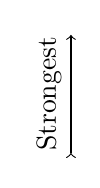
\begin{tikzpicture}
            \draw[->] (0,0) edge node [left]{\rotatebox{90}{Strongest}} (0, 1.5);
        \end{tikzpicture}} &
        Singleton GAC & maxRPWC \\
        \cline{2-3}
        & \multicolumn{2}{c|}{GAC} \\
        \cline{2-3}
        & Bound consistency & Forward checking \\
        \cline{2-3}
    \end{tabular}
    \caption{Relative stringths of the consistencies}
\end{table}


\subsection{Filtering consistencies}

if $x$ is a domain filtering consistency, a propagator for $x$ will :
from CSP(X, D, X) 
\begin{itemize}
    \item return (X, D', C) such that
        \begin{itemize}
            \item D' $\subseteq$ D
            \item (X, D, C) and (X, D', C) equivalent
            \item D' is a nonempty partial solution
            \item (X, D', C) respect $x$
        \end{itemize}
    \item return \textcolor{red}{fail} if no such CSP exists.

        $\to$ not possible to satisfy consistency = unsatisfiable CSP
\end{itemize}


\subsection{Arc consistency}
Strongest filtering when considering constraints in isolation.

\paragraph{GAC $\neq$ Satisfiability} : A CSP that is GAC may not
be satisfiable

\paragraph{AC} A \underline{binary} constraint $c$ on $x, y$ is AC iff
\begin{lstlisting}[mathescape]
    $\forall a \in D(x), \exists b \in D(y) : (a,b) \in c$ 
    $\forall a \in D(x), \exists b \in D(y) : (a,b) \in c$
\end{lstlisting}

$\to$ It means that all the value of variables are \textbf{supported}

\paragraph{GAC} A constraint $c$ is GAC iff
\begin{lstlisting}[mathescape]
    $\forall x_i \in scope(c)$
        $\forall a_i \in D(x_i)$
            $\exists a_1,..., a_{i-1}, a_{i+1},..., a_r $
                    $\in D(x_1) \times ... \times D(x_{i-1}) \times D(x_{i+1}) \times ... \times D(x_r)$
                $(a_1,...,a_r) \in c$

\end{lstlisting}

\subsubsection{Algorithm}
\begin{lstlisting}[mathescape, caption=GAC]
propagateGAC(Q){
    while(Q $\neq$ $\emptyset$){
        c = popCtrt(Q)
        $\Delta$ = c.propagate()
        for((x,a) $\leftarrow$ $\Delta$){
            removeValue(a,D(x))             
            for(c $\leftarrow$ C/{c} if c.scope contains x){
                if(! Q contains c)
                    Q += c
            }
        }
    }
}
\end{lstlisting}


\subsection{Bound consistency}
GAC can be costly, so a other consistency is to only search support for bound.
 $\to$ all valuyes between min and max considered in the domain.
 
\paragraph{BC} A \underline{binary} constraint $c$ on $x, y$ is BC iff
\begin{lstlisting}[mathescape]
    $\forall a \in { min(D(x)), max(D(x))}, \exists b \in [min(D(y)), max(D(y))]: c(a,b)$
    $\forall b \in { min(D(y)), max(D(y))}, \exists a \in [min(D(x)), max(D(x))]: c(a,b)$
\end{lstlisting}

\paragraph{BC} A constraint $c$ is BC iff
\begin{lstlisting}[mathescape]
    $\forall x_i \in scope(c)$
        $\forall a_i \in { min(D(y)), max(D(y))}$
            $\exists a_1,..., a_{i-1}, a_{i+1},..., a_r $
                    $\in D*(x_1) \times ... \times D*(x_{i-1}) \times D*(x_{i+1}) \times ... \times D*(x_r):$
                $c(a_1,..., a_r)$

$D*(x_k) = [min(D(x_k)), max(D(x_k))]$
\end{lstlisting}

\subsubsection{Algorithm}
\begin{lstlisting}[mathescape, caption=BC]
propagateGAC(Q){
    while(Q $\neq$ $\emptyset$){
        c = popCtrt(Q)
        $\Delta$ = c.propagate()
        for((x,a) $\leftarrow$ $\Delta$){
            removeValue(a,D(x))             
=>          if(a > x.max || a < x.min){
                for(c $\leftarrow$ C/{c} if c.scope contains x){
                    if(! Q contains c)
                        Q += c
                }
        }
    }
}
\end{lstlisting}

\subsection{Forward checking}

It's like a GAC at the end.
 
\paragraph{FC} A constraint $c$ is FC iff
\begin{lstlisting}[mathescape]
    if $\forall x_i \in scope(c):$ $D(x_i) = {v_i} then c(v_1, ..., v_r)$
    if all but one variable assigned: $c$ is GAC
\end{lstlisting}

\subsubsection{Algorithm}
\begin{lstlisting}[mathescape, caption=FC]
propagateGAC(Q){
    while(Q $\neq$ $\emptyset$){
        c = popCtrt(Q)
        $\Delta$ = c.propagate()
        for((x,a) $\leftarrow$ $\Delta$){
            removeValue(a,D(x))             
>          if($\#D(x) == 1$){
                for(c $\leftarrow$ C/{c} if c.scope contains x){
                    if(! Q contains c)
                        Q += c
                }
        }
    }
}
\end{lstlisting}


\subsection{Singleton consistencies}

\paragraph{Singleton} A CSP (\textsc{X, D, C}) is singleton $X_{Consistent}$ iff
\begin{lstlisting}[mathescape]
    $\forall x \in X, \forall a \in D(x):$ the CSP(\textsc{X, $D_{x=a}$, C) can be made S consistent
\end{lstlisting}

$D_{x=a} = D$ where $D(x)={a}$

\paragraph{Singleton GAC} A constraint $c$ is singleton GAC iff
\begin{lstlisting}[mathescape]
    $\forall x \in X, \forall a \in D(x):$ the CSP(\textsc{X, $D_{x=a}$, C) can be made GAC
\end{lstlisting}

In world, the singleton check the consistency after \textit{assign} a value to
a variable.


\subsection{Max Restricted Pairwise consistency}

\begin{itemize}
    \item Each literal has one support in each constraint c
    \item This support is extensible to the constrains linked with c

    \item[$\to$] Two constraints are linked if they share variable
\end{itemize}

\paragraph{maxRPWC} A constraint $c$ is maxRPWC iff
all literals $(x, a)$ have a \textbf{pairwise consistent support} in every 
constraints $c$ such that x $\in$ scope(c)

\paragraph{ }A pairwise consistent support for $(x,a)$ on constraint c is :
\begin{lstlisting}[mathescape]
    a valid tuple $\gamma \in c$ such that $\gamma(x) = a$
    $\forall c_j \neq c :$ scope(c) $\cap$ scope($c_j$) $\neq \emptyset$ : $\exists$ valid $\omega \in c_j$ such that
                $\gamma$(scope(c) $\cap$ scope($c_j$)) = $\omega$(scope(c) $cap$ scope($c_j$))
\end{lstlisting}

\begin{figure}[!h]
    \centering
    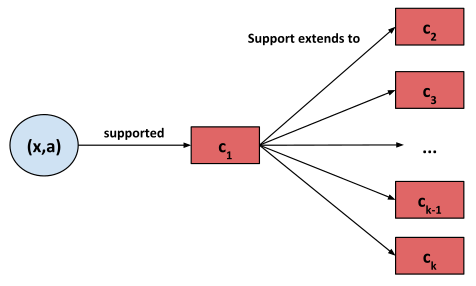
\includegraphics[width=8cm]{img/maxRPWC}
    \caption{maxRPWC}
\end{figure}

\subsubsection{Example}
\begin{figure}[!h]
\begin{tikzpicture}
    \node (A) {D(x) = \{0, 1\}};
    \node (B) [right=2cm of A] {D(y) = \{1, 2\}};
    \node (C) [right=2cm of B] {D(z) = \{1, 2\}};

    \node (D) [below right=1cm and 1cm of A] {$c_1$: x = |y-z|};
    \node (E) [below right=1cm and 1cm of B] {$c_2$: y $\neq$ z};
\end{tikzpicture}
\caption{Example CSP GAC but not maxRPWC}
\end{figure}

\begin{itemize}
    \item The support for (x,0) in $c_1$ are ((y,1), (z,1)) and ((y,2),(z,2))
    \item but those supports are not extensible to $c_2$ 
    \item[$\to$] (x,0) will never be part of a solution
\end{itemize}
                                                         
\section{Consistencies/Propagations algorithm and constraints}

\begin{figure}[!h]
    \centering
    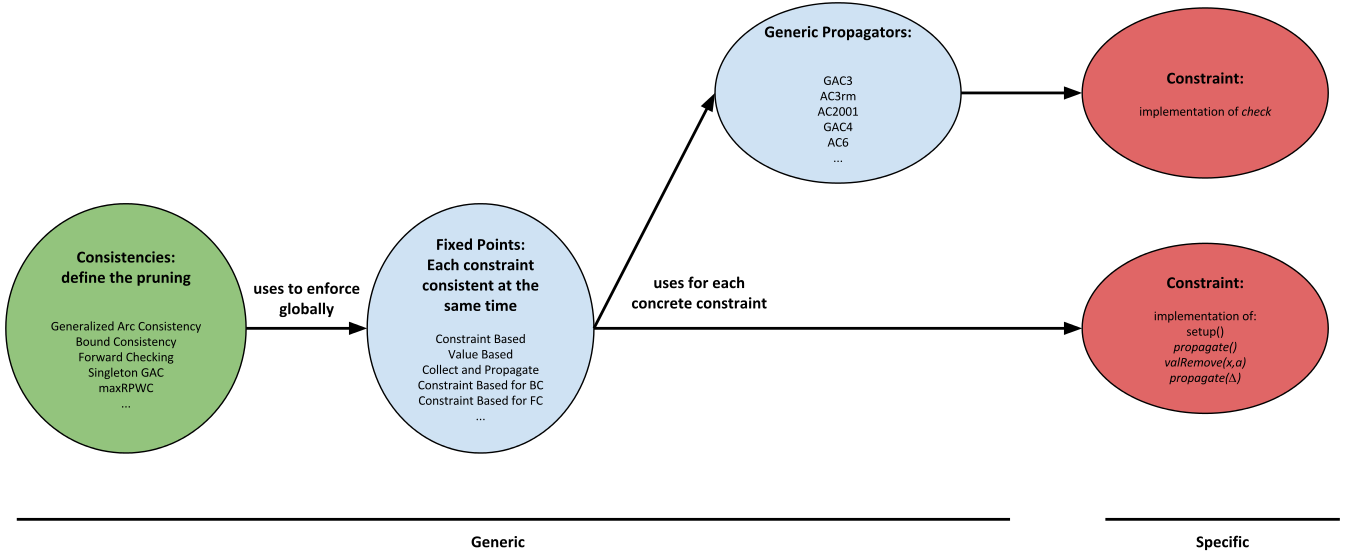
\includegraphics[width=\linewidth]{img/consistency-propagation.png}
    \caption{Link}
\end{figure}

\subsection{Mixing constraint}

The idea is to mix for different constraints : different consistencies and different fixed points

\begin{tabular}{m{1cm}cm{6cm}cm{6cm}}
    \textbf{Global fixed point}
    & = &
    \begin{itemize}
        \item ensuring each queue ($C_{CB}, C_{CV}, C_{CB-BC}, CP_{CB-FC}$) is empied
        \item ensuring impacted constraints put on the right queue
    \end{itemize}
    & 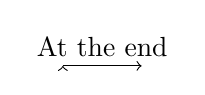
\begin{tikzpicture}
        \draw[->] (0,0) edge node[above] {At the end} (1,0); 
    \end{tikzpicture}
    &
    \begin{itemize}
        \item each constraint respects its consistency
        \item all at the same time
    \end{itemize}
\end{tabular}


\subsection{Mixing in practice}
\begin{enumerate}
    \item Constraints register to particular events on the domains/variables :
        \begin{itemize}
            \item a \textbf{value} has been removed (\textit{VB or collect \& propagate})
            \item the \textbf{domains} have been changed (\textit{CB})
            \item the \textbf{bounds} of the domains have changed (\textit{CB for BC})
            \item a variables is \textbf{assigned} (\textit{CB for FC})
        \end{itemize}

    \item When event occurs in a domain/variable :
        \begin{itemize}
            \item constraints put on the right queue and fixed point resumed
            \item makes the bridge beteween different queues
        \end{itemize}
\end{enumerate}



\section{Search}

\paragraph{Search tree} is defined by 
\begin{itemize}
    \item One CSP
    \item Branching
    \item Variable/value selection heuristic
    \item Exploration strategy
\end{itemize}

\paragraph{Tree} The tree is constructed during exploration and only the current
node in memory (DFS). The alternative decisions is memorized.

\paragraph{Node expansion}
Subdivision of a CSP into smaller CSP such that the union of the small CSP
is equivalent to the original.


\subsection{Depth first backtraking search}

\begin{itemize}
    \item Based on 
        \begin{enumerate}
            \item \textbf{stack of sets of decision}
            \item \textbf{stack of restoration states}
        \end{enumerate}
    \item Backtracking restores: 
        \begin{enumerate}
            \item Variables/domains
            \item Constraints
            \item Backtracked structures (ex: fistSupport)
        \end{enumerate}
\end{itemize}

\begin{lstlisting}[caption=Depth First backtracking search]
while (! decisionStack.isEmpty) {
    val decisionsOfNode = decisionStack.pop()

    val decision = decisionsOfNode.pop()
    if( decision.hasNext() )
        pushState()

    applyDecision(decision)

    if (!isFailed() ){
        val isExpandable = expand(branching)
        if (! isExpandable) {
            solFound()
            popState()
        }
    } else {
        popState()
    }
}
\end{lstlisting}

\subsubsection{Trailing}
In opposition to copying the node in order to perform backtracking, 
trailing only store the \textbf{modification}.

\paragraph{Trail level}
Trailed operations are marked with an integer which is increase!

\paragraph{Restoring} undo all operations with trail level greater than
desired set the trail level to desired one.


\subsection{Branching strategy}

\paragraph{Completeness}: a branching strategy is \textbf{completeness}
if the union of the child CSPs is the parent CSP

\subsubsection{Strategies}
\begin{tabular}{m{6cm}m{6cm}}
    \begin{itemize}
        \item binary labelling
    \end{itemize}
    &
    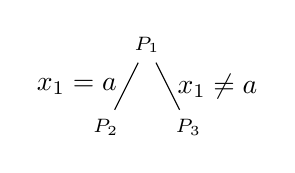
\begin{tikzpicture}[scale=0.7]
        \node[] {\scriptsize$P_1$} child{ node[] {\scriptsize$P_2$} 
        edge from parent node[above, left] {$x_1 = a$}}
        child { node[] {\scriptsize$P_3$} 
        edge from parent node[above, right] {$x_1 \neq a$}};

    \end{tikzpicture}
    \\
    \begin{itemize}
        \item n-ary labelling
    \end{itemize}
    &
    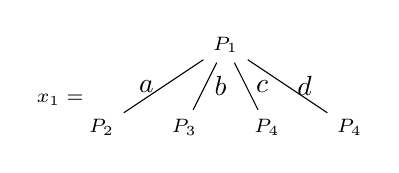
\begin{tikzpicture}[scale=0.7]
        \node[] {\scriptsize$P_1$} child{ node[] {\scriptsize$P_2$} 
        edge from parent node[above, left] {$a$}}
        child { node[] {\scriptsize$P_3$} 
        edge from parent node[above, right] {$b$}}
        child { node[] {\scriptsize$P_4$} 
        edge from parent node[above, right] {$c$}}
        child { node[] {\scriptsize$P_4$} 
        edge from parent node[above, right] {$d$}};

        \node at (-3,-1) {\scriptsize $x_1 =$};
    \end{tikzpicture}
    \\
    \begin{itemize}
        \item domain splitting
    \end{itemize}
    &
    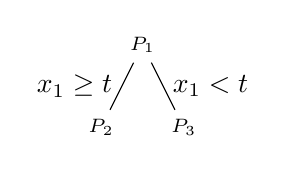
\begin{tikzpicture}[scale=0.7]
        \node[] {\scriptsize$P_1$} child{ node[] {\scriptsize$P_2$} 
        edge from parent node[above, left] {$x_1 \geq t$}}
        child { node[] {\scriptsize$P_3$} 
        edge from parent node[above, right] {$x_1 < t$}};

    \end{tikzpicture}
    \\
\end{tabular}

\subsubsection{Heuristics}
 
\begin{enumerate}
    \item Select a variable
    \item Ordering the values
\end{enumerate}

\paragraph{First fail principle}: choose first a variable that is more likely to fail

(Consider the most difficult parts of the CSP first)

\paragraph{Best first principle}: Choose first a value that is more likely to succeed

\paragraph{High impact of the first decisions}

\subsection{Variable ordering heuristics}

\subsection{Value ordering heuristics}

\subsection{Exploration strategies}

\subsection{Constraint optimization problem}

\section{Examen questions}

\begin{enumerate}
    \item \begin{itemize}
            \item Formal definition of CSP
            \item Formal definition of COP
            \item Definition of a constraint
            \item Principle of search in CP
            \item Current DOmain
            \item Communication in CP
            \item Computational model
        \end{itemize}
    \item 
    \item \begin{itemize}
            \item Consistency
            \item Definition of GAC
            \item Value based fixed point
            \item (G)AC3, AC3rm, AC2001, (G)AC4, AC6
            \item Complexities
            \item Invariant on their data structure
        \end{itemize}
    \item \begin{itemize}
            \item Fixed point: algorithms, commonalities, differences
            \item Definitions of consistencies : BC, FC, Singleton consitencies, 
                Singleton GAC, maxRPWC
            \item Relative strengths of consistencies
            \item Global view on propagation in CP
            \item An algorithm for a consistency inside a fixed point
                for a constraint
            \item How to mix consistencies
        \end{itemize}

\end{enumerate}


\end{document}
